%\documentstyle[epsf,twocolumn]{jarticle}       %LaTeX2e仕様
%\documentclass[twocolumn]{jarticle}     %pLaTeX2e仕様(platex.exeの場合)
\documentclass[onecolumn]{ujarticle}   %pLaTeX2e仕様(uplatex.exeの場合)
%%%%%%%%%%%%%%%%%%%%%%%%%%%%%%%%%%%%%%%%%%%%%%%%%%%%%%%%%%%%%%
%%
%%  基本バージョン
%%
%%%%%%%%%%%%%%%%%%%%%%%%%%%%%%%%%%%%%%%%%%%%%%%%%%%%%%%%%%%%%%%%
\setlength{\topmargin}{-45pt}
%\setlength{\oddsidemargin}{0cm}
\setlength{\oddsidemargin}{-7.5mm}
%\setlength{\evensidemargin}{0cm}
\setlength{\textheight}{24.1cm}
%setlength{\textheight}{25cm}
\setlength{\textwidth}{17.4cm}
%\setlength{\textwidth}{172mm}
\setlength{\columnsep}{11mm}

%\kanjiskip=.07zw plus.5pt minus.5pt

% 【節が変わるごとに (1.1)(1.2) … (2.1)(2.2) と数式番号をつけるとき】
%\makeatletter
%\renewcommand{\theequation}{%
%\thesection.\arabic{equation}} %\@addtoreset{equation}{section}
%\makeatother

%\renewcommand{\arraystretch}{0.95} 行間の設定
%%%%%%%%%%%%%%%%%%%%%%%%%%%%%%%%%%%%%%%%%%%%%%%%%%%%%%%%
%\usepackage{graphicx}   %pLaTeX2e仕様(\documentstyle ->\documentclass)
\usepackage[dvipdfmx]{graphicx}
\usepackage{subcaption}
\usepackage{multirow}
\usepackage{amsmath}
\usepackage{url}
\usepackage[bb=boondox]{mathalfa}
\usepackage{listings}
\newcommand{\argmax}{\mathop{\rm arg~max}\limits}
\newcommand{\argmin}{\mathop{\rm arg~min}\limits}

\lstset{%
  language={Python},
  basicstyle={\small},%
  identifierstyle={\small},%
  commentstyle={\small\itshape},%
  keywordstyle={\small\bfseries},%
  ndkeywordstyle={\small},%
  stringstyle={\small\ttfamily},
  frame={tb},
  breaklines=true,
  columns=[l]{fullflexible},%
  numbers=left,%
  xrightmargin=0zw,%
  xleftmargin=3zw,%
  numberstyle={\scriptsize},%
  stepnumber=1,
  numbersep=1zw,%
  lineskip=-0.5ex%
}

%%%%%%%%%%%%%%%%%%%%%%%%%%%%%%%%%%%%%%%%%%%%%%%%%%%%%%%%
\begin{document}

	%bibtex用の設定
	%\bibliographystyle{ujarticle}
	\noindent

	\hspace{1em}
	2020 年 12 月 4 日
	ゼミ資料
	\hfill
	M2 寺内 光

	\vspace{2mm}

	\hrule

	\begin{center}
		{\Large \bf 進捗報告}
	\end{center}

	\hrule
	\vspace{3mm}

	% ‚ここから 文章 Start!
	\section{今週やったこと}
	漫画データに対する適用実験, 引き継ぎ準備, AAAI preprint 準備

  \section{漫画データに対する適用実験}
  漫画の作品名識別, 入れ替え識別に対する TDGA AA の適用実験をした.表 \ref{tab:num_data} に各作品のデータ数およびクラスラベルを示す.

  \begin{table}[h]
  	\centering
  	\caption{各作品の全データおよび対応ラベル}
  	\label{tab:num_data}
  	\begin{tabular}{|c||c|c|} \hline
      作品名&データ数&ラベル \\ \hline
      少年漫画タッチ&80&0\\ \hline
      あくはむ&676&1\\ \hline
      高校の人達&908&2\\ \hline
      OLランチ&828&3\\ \hline
      徹さん&520&4\\ \hline
      幼稚園ぼうえい組&360&5\\ \hline
  	\end{tabular}
  \end{table}

  表 \ref{tab:result_experiments} に結果を示す.ばらつきは大きいものの, 適切な温度設定において漫画データセットにおいても精度の向上が見られることが確認できた.

  \begin{table}[h]
		\centering
		\caption{作品名識別, 入れ替え識別 Test accuracy(\%)}
		\label{tab:result_experiments}
		\begin{tabular}{l||c c c} \hline
		  &Baseline&Baseline(Cutout)&TDGA AA\\ \hline
      作品名識別&94.38$\pm$1.30 &95.03$\pm$1.05&95.86$\pm$0.53\\
      入れ替え識別&75.76$\pm$1.45 &75.92$\pm$0.53&77.96$\pm$0.58\\
		\end{tabular}
	\end{table}

  図 \ref{fig:change_temperature_comic}, \ref{fig:change_temperature_fourscene} に作品名識別および入れ替え識別の温度変化に対する識別率を示す.

  \begin{figure}[h]
  \centering
  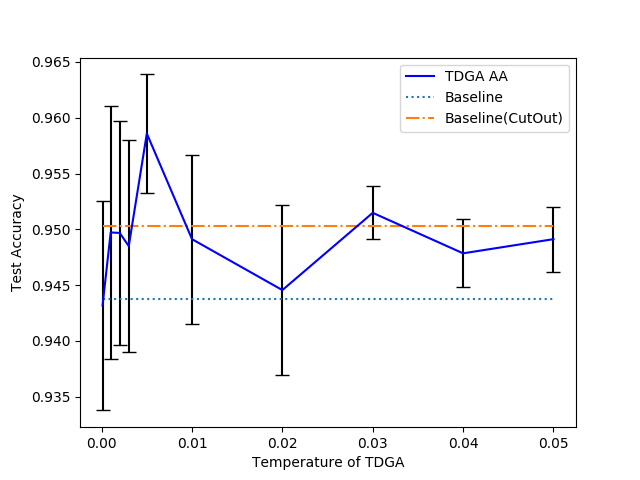
\includegraphics[width=0.6\columnwidth]{figure/exp_change_temperature_comic.png}
  \caption{温度に対する作品名識別の識別率の変化}
  \label{fig:change_temperature_comic}

  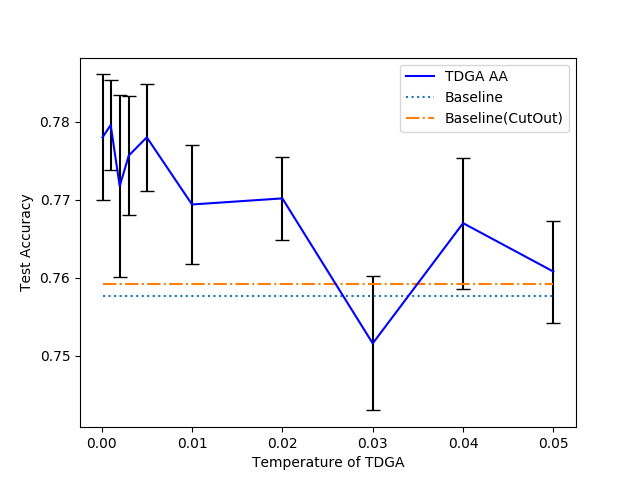
\includegraphics[width=0.6\columnwidth]{figure/exp_change_temperature_fourscene.png}
  \caption{温度に対する入れ替え識別の識別率の変化}
  \label{fig:change_temperature_fourscene}
  \end{figure}

  図 \ref{fig:num_transforms_comic}, \ref{fig:num_transforms_fourscene} に作品名識別および入れ替え識別における最終エントロピーと個体数を示す.棒グラフの青色は最終世代の拡張で,橙色はそのうち採用された個数を示す.

  \begin{figure}[h]
  \centering
  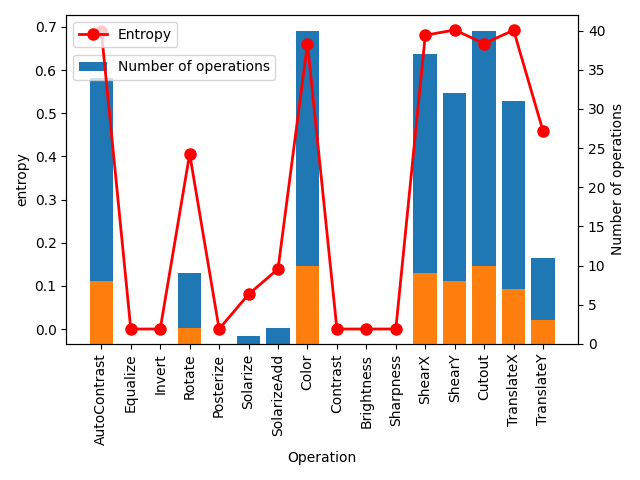
\includegraphics[width=0.6\columnwidth]{figure/num_transforms_comic.png}
  \caption{作品名識別におけるエントロピーと個体数}
  \label{fig:num_transforms_comic}

  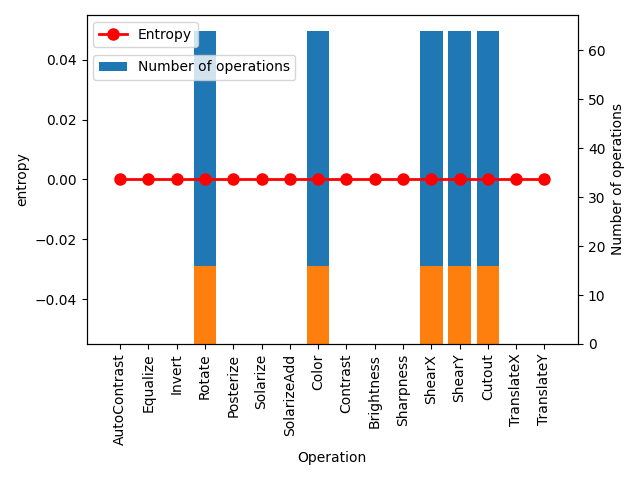
\includegraphics[width=0.6\columnwidth]{figure/num_transforms_fourscene.png}
  \caption{入れ替え識別におけるエントロピーと個体数}
  \label{fig:num_transforms_fourscene}
  \end{figure}

  作品名識別においては温度設定による拡張の有効性がある程度示せた.しかし入れ替え識別においては,初期収束によって全個体が同一になってしまっている.これは特徴抽出部の重みを固定しているためあまり拡張が効かなかったことが原因ではないかと考えている.こういったデータのためにも, ある程度温度をどのように決めるかについての調整方法は必要だと考えられる.


  表 \ref{tab:exp_title_measure_before}, \ref{tab:exp_title_measure_after} に作品名識別における指標値を示す.TDGA AA ありとなしの場合を比べると各クラス毎に F-1 スコアがあがっていることがわかる.

  \begin{table}[h]
  	\centering
  	\caption{作品名識別 指標 (Baseline)}
  	\vspace{-3mm}
  	\label{tab:exp_title_measure_before}
  	\begin{tabular}{|c|c|c|c|c|} \hline
  		クラスラベル&Precision&Recall&F-1&サンプル数\\ \hline\hline
  		0&1.00&1.00&1.00&8\\ \hline
  		1&0.97&0.88&0.92&68\\ \hline
  		2&0.94&1.00&0.97&91\\ \hline
  		3&0.94&0.99&0.96&83\\ \hline
  		4&1.00&0.83&0.91&52\\ \hline
      5&0.85&0.97&0.91&36\\ \hline
  		macro avg&0.95&0.94&0.95&338\\ \hline
  		weighted avg&0.95&0.94&0.94&338\\ \hline
  		accuracy&&&&0.9438\\ \hline
  	\end{tabular}
  \end{table}

  \begin{table}[h]
  	\centering
  	\caption{作品名識別 指標 (TDGA)}
  	\vspace{-3mm}
  	\label{tab:exp_title_measure_after}
  	\begin{tabular}{|c|c|c|c|c|} \hline
  		クラスラベル&Precision&Recall&F-1&サンプル数\\ \hline\hline
  		0&1.00&1.00&1.00&8\\ \hline
  		1&0.97&0.91&0.94&68\\ \hline
  		2&0.95&0.99&0.97&91\\ \hline
  		3&0.98&0.96&0.97&83\\ \hline
  		4&1.00&0.90&0.95&52\\ \hline
      5&0.86&1.00&0.92&36\\ \hline
  		macro avg&0.96&0.96&0.96&338\\ \hline
  		weighted avg&0.96&0.96&0.96&338\\ \hline
  		accuracy&&&&0.9556\\ \hline
  	\end{tabular}
  \end{table}

  表 \ref{tab:exp_fourscene_measure_before}, \ref{tab:exp_fourscene_measure_after} に入れ替え識別における指標値を示す.入れ替え識別においてはクラス 0 の F-1 スコアが大きく上がり, 逆にクラス 1 の F-1 スコアが少し下がっていることがわかる.これは今までクラス 0 と クラス 1 の分類で多くがクラス 1 に分類されてしまっていたのが緩和された影響であると考察できる.

  \begin{table}[h]
  	\centering
  	\caption{入れ替え識別 指標 (Baseline)}
  	\vspace{-3mm}
  	\label{tab:exp_fourscene_measure_before}
  	\begin{tabular}{|c|c|c|c|c|} \hline
  		クラスラベル&Precision&Recall&F-1&サンプル数\\ \hline\hline
  		0&0.71&0.46&0.56&85\\ \hline
  		1&0.66&0.81&0.73&85\\ \hline
  		2&0.89&1.00&0.94&85\\ \hline
  		macro avg&0.75&0.76&0.74&255\\ \hline
  		accuracy&&&&0.7569\\ \hline
  	\end{tabular}
  \end{table}

  \begin{table}[h]
  	\centering
  	\caption{入れ替え識別 指標 (TDGA)}
  	\vspace{-3mm}
  	\label{tab:exp_fourscene_measure_after}
  	\begin{tabular}{|c|c|c|c|c|} \hline
  		クラスラベル&Precision&Recall&F-1&サンプル数\\ \hline\hline
  		0&0.67&0.68&0.67&85\\ \hline
  		1&0.74&0.65&0.69&85\\ \hline
  		2&0.89&0.99&0.94&85\\ \hline
  		macro avg&0.77&0.77&0.77&255\\ \hline
  		accuracy&&&&0.7765\\ \hline
  	\end{tabular}
  \end{table}

  \section{-12/15 のタスク}
  AAAI の preprint 準備.検証データに対する精度を見るのと SGA との比較をやってみる.

	% 参考文献リスト
	% \bibliographystyle{unsrt}
	% \bibliography{2020_11_6}
\end{document}
